\subsection{Double Slit Interference}

\begin{enumerate}
    \item Two closely spaced parallel slits acts as \textbf{coherent sources of waves} - they emit light waves with a \textbf{constant phase difference} and the \textbf{same frequency}.
        \begin{itemize}
            \item A \textbf{laser beam} could be used instead of a light bulb and a single slit.
        \end{itemize}
    \item \textbf{Young's fringes} - \textbf{evenly spaced}, alternative bright and dark fringes can be seen on a white screen where the diffracted light from the double slits \textbf{overlap}.
\end{enumerate}

The fringes are formed due to the \textbf{interference of light} from the slits.
\begin{itemize}
    \item Bright fringe is formed where light from one slit \textbf{reinforces light from the other slit}.
        \begin{itemize}
            \item The light waves from each slit arrive \textbf{in phase} with each other.
        \end{itemize}
    \item Dark fringe is formed where light from one slit \textbf{cancels light from the other slit}.
        \begin{itemize}
            \item The light waves from each slit arrive \textbf{180 deg out of phase}.
        \end{itemize}
\end{itemize}

\textbf{Fringe separation} is the distance from the centre of the of the bright fringe to the centre of the next bright fringe.
$$\text{fringe separation}\ w=\frac{\lambda D}{s}$$
where $s$ is the \textbf{slit spacing} and $D$ is the distance from the slits to the screen.

\subsubsection*{Theory of Double Slit Equation}

\begin{center}
    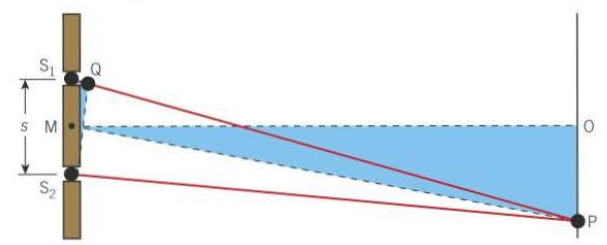
\includegraphics[width=5cm]{img/slits}
\end{center}

\begin{itemize}
    \item \textbf{Reinforcement} at $P$ if the \textbf{path difference} $S_1P-S_2P=m\lambda$
    \item \textbf{Cancellation} at $P$ if the \textbf{path difference} $S_1P-S_2P=\left(m+\frac{1}{2}\right)\lambda$
\end{itemize}
where $m=0,1,2,\dots$

From the diagram
\begin{align*}
    \frac{S_1Q}{S_1S_2}&=\frac{OP}{OM}\\
    \frac{m\lambda}{s}&=\frac{mw}{D}\\
    w&=\frac{\lambda D}{s}
\end{align*}
